%%%%%%%%%%%%%%%%%%%%%%%%%%%%%%%%%%%%%%%%%%%%%%%%%%%%%%%%%%%%%%%%
%% Dissertation Presentation about the M.Sc. Thesis
%%%% Siegel, Shriki, Tolpin. "Computational Approaches to Seizure Forecasting" Thesis defenese,
%%
%% Presented for Computer Science M.Sc. Panel @ Ben Gurion University
%% Slides and notes written by Noam Siegel <noamsglrkr@gmail.com>
%%
%% ---------------------------------------------------------- %%
%% Licensed under Creative Commons Attribution-ShareAlike 3.0 %%
%% http://creativecommons.org/licenses/by-sa/3.0/             %%
%%%%%%%%%%%%%%%%%%%%%%%%%%%%%%%%%%%%%%%%%%%%%%%%%%%%%%%%%%%%%%%%
%%%%%%%%%%%%%%%%%%%%%%%% PREAMBLE
\documentclass[t]{beamer}
% \usepackage{pgfpages}
% \usepackage{handoutWithNotes}
% \pgfpagesuselayout{4 on 1 with notes}[a4paper,border shrink=5mm]
% \pgfpagesuselayout{4 on 1}[a4paper,border shrink=5mm]
%%%%%%%%%%%%%%%%%%%%%%%% PREAMBLE
\usepackage[
    type={CC},
    modifier={by-nc-sa},
    version={3.0},
]{doclicense}

\usepackage[T1]{fontenc}
% \usepackage[utf8]{inputenc}  % usually redundant since this is default anyways
% \UseRawInputEncoding
\usepackage{graphicx, calligra}
\graphicspath{ {./figs/} }
\usepackage{tikz}
\usetikzlibrary {arrows.meta,bending,positioning}
\usepackage{latexsym,amsmath,xcolor,multicol,booktabs,calligra}
\usepackage{graphicx,listings,stackengine}
\usepackage{BGU}
\usepackage{subfigure}
\usepackage[font=tiny,labelfont=bf]{caption}
\usepackage{appendixnumberbeamer}  %  don't count appendix pages in slide count
\usepackage{cancel}  % strike through diagonally
% \usepackage{todonotes}
% \presetkeys{todonotes}{inline}{}  % for beamer
% \usepackage{biblatex}
% \usepackage{bibentry}
\usepackage[sort]{natbib}

% defs
\newcommand{\prob}{\mathbb{P}}
\def\cmd#1{\texttt{\color{red}\footnotesize $\backslash$#1}}
\def\env#1{\texttt{\color{blue}\footnotesize #1}}
\definecolor{lightgray}{gray}{0.75}
\definecolor{lightgreen}{HTML}{a5cf90}
\definecolor{lightpurple}{HTML}{a49cbc}
\definecolor{halfgray}{gray}{0.55}
\definecolor{halfgreen}{RGB}{204, 255, 102}
\definecolor{deepblue}{rgb}{0,0,0.5}
\definecolor{deepred}{rgb}{0.6,0,0}
\definecolor{deepgreen}{rgb}{0,0.5,0}
\definecolor{crimson}{rgb}{0.863, 0.078, 0.235}
\definecolor{peach}{rgb}{100, 89.8, 70.6}
\definecolor{applegreen}{rgb}{0.55, 0.71, 0.0}
\definecolor{grape}{HTML}{2f2b72}

\lstset{
    basicstyle=\ttfamily\small,
    keywordstyle=\bfseries\color{deepblue},
    emphstyle=\ttfamily\color{deepred},    % Custom highlighting style
    stringstyle=\color{deepgreen},
    numbers=left,
    numberstyle=\small\color{halfgray},
    rulesepcolor=\color{red!20!green!20!blue!20},
    frame=shadowbox,
}

%%%%%%%%%%%%%%%%%%%%%%%% BEAMER NOTES
% https://gist.github.com/andrejbauer/ac361549ac2186be0cdb
% These slides also contain speaker notes. You can print just the slides,
% just the notes, or both, depending on the setting below. Comment out the want
% you want.

% \setbeameroption{hide notes} % Only slides
% \setbeameroption{show only notes} % Only notes
\setbeameroption{show notes on second screen=right} % Both

% To give a presentation with the Skim reader (http://skim-app.sourceforge.net) on OSX so
% that you see the notes on your laptop and the slides on the projector, do the following:
% 
% 1. Generate just the presentation (hide notes) and save to slides.pdf
% 2. Generate only the notes (show only nodes) and save to notes.pdf
% 3. With Skim open both slides.pdf and notes.pdf
% 4. Click on slides.pdf to bring it to front.
% 5. In Skim, under "View -> Presentation Option -> Synhcronized Noted Document"
%    select notes.pdf.
% 6. Now as you move around in slides.pdf the notes.pdf file will follow you.
% 7. Arrange windows so that notes.pdf is in full screen mode on your laptop
%    and slides.pdf is in presentation mode on the projector.

% Give a slight yellow tint to the notes page
\setbeamertemplate{note page}{\pagecolor{yellow!5}\insertnote}\usepackage{palatino}


%%%%%%%%%%%%% BEAMER SETTINGS %%%%%%%%%%%%%%
% \AtBeginSection[]
% {
% \begin{frame}<beamer>
% \frametitle{Plan}
% \tableofcontents[currentsection]
% \end{frame}
% }

% \AtBeginSubsection[] % Do nothing for \subsection*
% {
% % \begin{frame}<beamer>
% % \frametitle{Outline}
% % \tableofcontents[currentsection,currentsubsection]
% % \end{frame}
% }

%%% MACROS
\usepackage{svg}
\usepackage{pdfpages}
\usepackage{amsmath}
\usepackage{bm}
\newtheorem{reminder}{Reminder}

\theoremstyle{definition}
\newtheorem*{fct}{Fact}
\newtheorem*{hwv}{However}
\DeclareMathOperator*{\argmax}{arg\,max}
\DeclareMathOperator*{\argmin}{arg\,min}

\pdfstringdefDisableCommands{% allows the use of \baselineskip despite using hyperref
    \def\baselineskip{}%
}
%%%% Allows repeating frame contents (duplicating boxes)
% https://tex.stackexchange.com/questions/107237/repeating-frame-contents
\newcommand\dupbox[2][]{%
\begin{block}{\duptitle}
\begin{minipage}{\linewidth}
\duptext
\end{minipage}
\end{block}
\begin{block}{#1}
\begin{minipage}{\linewidth}
#2
\end{minipage}
\end{block}
\gdef\duptext{#2}
\gdef\duptitle{#1}
}

\gdef\duptext{Initial text}
\gdef\duptitle{}



%%%%% THEME
% \usetheme{Boadilla}
% \usetheme{Madrid}
% \usecolortheme{default}


%% Enable license helpers
%%%%%%%%%%%%%%%%%%%%%%%%%%%%%%%%%%%%%%%%%%%%%%%%%%%%%%%%%%%%%%%%
%% ccBeamer 0.1, 2007-07-02                                   %%
%% Written by Sebastian Pipping <webmaster@hartwork.org>      %%
%% ---------------------------------------------------------- %%
%% Licensed under Creative Commons Attribution-ShareAlike 3.0 %%
%% http://creativecommons.org/licenses/by-sa/3.0/             %%
%%%%%%%%%%%%%%%%%%%%%%%%%%%%%%%%%%%%%%%%%%%%%%%%%%%%%%%%%%%%%%%%


%% Images
\newcommand{\CcImageBy}[1]{%
	
\includegraphics[scale=#1]{creative_commons/cc_by_30.pdf}%
}
\newcommand{\CcImageCc}[1]{%
	
\includegraphics[scale=#1]{creative_commons/cc_cc_30.pdf}%
}
\newcommand{\CcImageDevNations}[1]{%
	
\includegraphics[scale=#1]{creative_commons/cc_dev_nations_30.pdf}%
}
\newcommand{\CcImageNc}[1]{%
	
\includegraphics[scale=#1]{creative_commons/cc_nc_30.pdf}%
}
\newcommand{\CcImageNd}[1]{%
	
\includegraphics[scale=#1]{creative_commons/cc_nd_30.pdf}%
}
\newcommand{\CcImagePd}[1]{%
	
\includegraphics[scale=#1]{creative_commons/cc_pd_30.pdf}%
}
\newcommand{\CcImageSa}[1]{%
	
\includegraphics[scale=#1]{creative_commons/cc_sa_30.pdf}%
}
\newcommand{\CcImageSampling}[1]{%
	
\includegraphics[scale=#1]{creative_commons/cc_sampling_30.pdf}%
}
\newcommand{\CcImageSamplingPlus}[1]{%
	
\includegraphics[scale=#1]{creative_commons/cc_sampling_plus_30.pdf}%
}


%% Groups
\newcommand{\CcGroupBy}[1]{% zoom
	\CcImageBy{#1}%
}
\newcommand{\CcGroupByNc}[2]{% zoom, gap
	\CcImageBy{#1}\hspace*{#2}\CcImageNc{#1}%
}
\newcommand{\CcGroupByNcNd}[2]{% zoom, gap
	\CcImageBy{#1}\hspace*{#2}\CcImageNc{#1}\hspace*{#2}\CcImageNd{#1}%
}
\newcommand{\CcGroupByNcSa}[2]{% zoom, gap
	\CcImageBy{#1}\hspace*{#2}\CcImageNc{#1}\hspace*{#2}\CcImageSa{#1}%
}
\newcommand{\CcGroupByNd}[2]{% zoom, gap
	\CcImageBy{#1}\hspace*{#2}\CcImageNd{#1}%
}
\newcommand{\CcGroupBySa}[2]{% zoom, gap
	\CcImageBy{#1}\hspace*{#2}\CcImageSa{#1}%
}
\newcommand{\CcGroupDevNations}[1]{% zoom
	\CcImageDevNations{#1}%
}
\newcommand{\CcGroupNcSampling}[2]{% zoom, gap
	\CcImageNc{#1}\hspace*{#2}\CcImageSampling{#1}%
}
\newcommand{\CcGroupPd}[1]{% zoom
	\CcImagePd{#1}%
}
\newcommand{\CcGroupSampling}[1]{% zoom
	\CcImageSampling{#1}%
}
\newcommand{\CcGroupSamplingPlus}[1]{% zoom
	\CcImageSamplingPlus{#1}%
}


%% Text
\newcommand{\CcLongnameBy}{Attribution}
\newcommand{\CcLongnameByNc}{Attribution-NonCommercial}
\newcommand{\CcLongnameByNcNd}{Attribution-NoDerivs}
\newcommand{\CcLongnameByNcSa}{Attribution-NonCommercial-ShareAlike}
\newcommand{\CcLongnameByNd}{Attribution-NoDerivs}
\newcommand{\CcLongnameBySa}{Attribution-ShareAlike}

\newcommand{\CcNote}[1]{% longname
	Slides licensed under the \textit{Creative Commons #1 3.0 License}.%
}


%%%% HEADER
\title[Weakly Supervised Bayesian Estimation of Seizure Likelihood]{Weakly Supervised Bayesian Estimation\\of Seizure Likelihood}
% \subtitle{Masters of Science -- Thesis Defense}
% \author{Noam Siegel}
% \institute[BGU]
% {Computer Science Department\\
% Faculty of Natural Sciences\\
% Ben Gurion University of the Negev}
% \author[shortname]{author1 \inst{1} \and author2 \inst{2}}
% \institute[shortinst]{\inst{1} affiliation for author1 \and %
                    %   \inst{2} affiliation for author2}

\author[Noam Siegel]{Noam Siegel \\ [\baselineskip] {\small {Supervised By} \and\\Dr. Oren Shriki \& Dr. David Tolpin}}

% \institute[BGU]{Ben-Gurion University of the Negev}
\institute[BGU]{
\includegraphics[height=1.2cm]{imgs/just-logo.png}\\Ben-Gurion University of the Negev}
% \setbeamerfont{institute}{size=\normalsize}

\date{\today}

%%%%%%%%%%%%% DOCUMENT %%%%%%%%%%%%%%
\begin{document}

%%%%%%%%%%%%% Title Page %%%%%%%%%%%%%%

\begin{frame}
	\titlepage
	\vfill
	\begin{center}
% 		\CcGroupByNcSa{0.83}{0.95ex}\\[.5ex]
% 		{\tiny\CcNote{\CcLongnameByNcSa}}
% 		\vspace*{-2.5ex}
	\end{center}
    % 	\note[item]{Thank the audience for being awake.}
	\note[item]{Prepare markers and eraser, erase the board. (20 minutes -t)}
	\note[item]{Reset the timer. (5 -t)}
	\note[item]{Begin welcome speech. (t)}
\end{frame}
%%%%%%%%%%%%% License %%%%%%%%%%%%%%


%%%%%%%%%%%%% TOC %%%%%%%%%%%%%%
\begin{frame}
	\frametitle{Outline}
	\tableofcontents
        \note[item]{t+1 : outline plan}
\end{frame}

%%%%%%%%%%%%% DOCUMENT %%%%%%%%%%%%%%
\section{Introduction}

%%%%%%%%%%%%% Preliminaries %%%%%%%%%%%%%%

% \subsection{Prerequisites}

% \begin{frame}{Prerequisites}
%         \todo{todo: add prerequisites}
% % 		\todo{add illustration of Probabilistic Inference in Graphical Models}
% % 		\todo{add illustration of Dynamic Bayesian Networks}
%         \note{for example: probabilistic inference, graphical models, dynamic bayesian networks}
% \end{frame}

%%%%%%%%%%%%%%%%%%%%%%%%%%%
\subsection{Motivation}

\begin{frame}<1-2>{Background}
    \only<1>{
    \begin{figure}
        \centering
        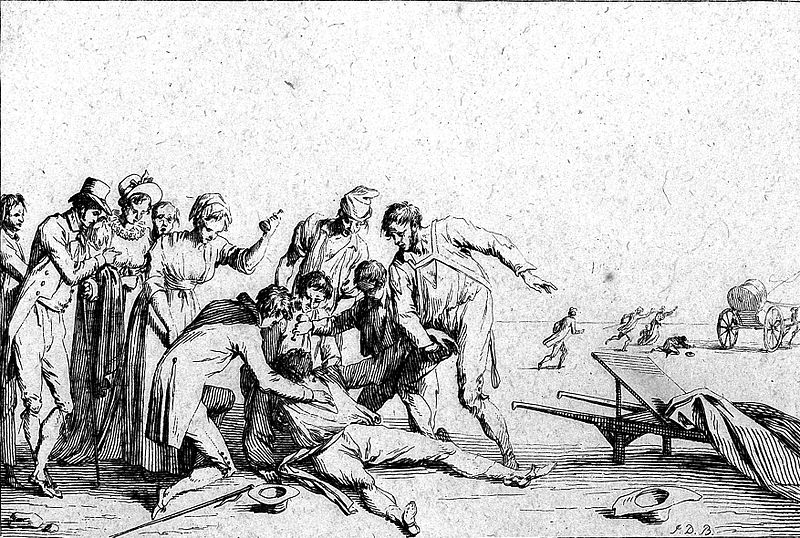
\includegraphics[width=0.7\textwidth]{figs/iconograph_epilepsy.jpg}
        \caption{18th century iconograph of an epilepsy seizure. Etched by J. Duplessi-Bertaux. Credit:  Wellcome Library, London. Licensed under the \href{https://creativecommons.org/licenses/by/4.0/deed.en}{Creative Commons Attribution 4.0 International license.}}
        \label{fig:my_label}
    \end{figure}
    }

    \only<2>{        
    
        % \begin{figure}[h]
        %     \centering
        %     \includegraphics[width=\textwidth]{c1Introduction/eeg_easy_pics.jpg}
        %     \Caption{Electroencephalography (EEG) art}{\\\href{https://www.flickr.com/photos/easy-pics/9408344706}{eeg} from The Clear Communication People, licensed under \href{https://creativecommons.org/licenses/by-nc-nd/2.0/}{CC BY-NC-ND 2.0}.\\
        %     EEG is a form of neuroimagery with high temporal accuracy. In the noninvasive setup, a wearable cap holds electrodes in contact with the scalp. The electric potentials induced by the brain are transmitted to a digital recording system for data analysis.}
        %     \label{fig:c1intro:eeg}
        % \end{figure}

    
        
        \begin{figure}
            \centering
            \includegraphics[width=0.7\textwidth]{figs/eeg_easy_pics.jpg}
            \caption{\href{https://www.flickr.com/photos/easy-pics/9408344706}{Electroencephalography (EEG) art}.\\From: The Clear Communication People. Licensed under: \href{https://creativecommons.org/licenses/by-nc-nd/2.0/}{CC BY-NC-ND 2.0}.\\
            }
            \label{fig:data}
        
        \end{figure}
    }


    
    \note<1->[item]{\url{https://commons.wikimedia.org/wiki/File:A\_group\_of\_people\_standing\_around\_a\_man\_having\_an\_epileptic\_Wellcome_L0005934.jpg}}
    \note<1->[item]{In this iconograph from the 18th century, we see a group of people standing around a man having an epileptic fit.}
    \note<1->[item]{Studies have shown that the biggest impediment to patients with epilepsy is the uncertainty and surprise factor of the seizures.}
    \note<2->[item]{EEG is a form of neuroimagery with high temporal accuracy. Seen here is a scalp eeg, based on a wearable cap which holds electrodes in contact with the head's surface. The electric potentials induced by the brain are recorded by a digital sampler for data analysis.}
\end{frame}





\begin{frame}<1-4>{Background \& Motivation}
    \only<1->{
    \centering
    \begin{tikzpicture}
          %%%%%%%%%% OUTPUT figures %%%%%%%%%%
        % \onslide<2->{\draw (4,0.5) circle (0.5cm);}
        \onslide<1->{\draw[fill=yellow] (4,0.5) circle (0.5cm);}
        \onslide<1->{\node[text width=1cm, align=center] at (4,1.5) {?};}
        \node[text width=1cm, align=center] at (4,0.5) {\LARGE f};
        
        % Draw the output rectangles
        \draw[fill=lightgreen] (6,1) rectangle (8,2);
        \draw[fill=lightpurple] (6,0) rectangle (8,-1);
        \node[text width=2cm, align=center] at (7,1.5) {seizure};
        \node[text width=2cm, align=center] at (7,-0.5) {not seizure};

        % Draw the output arrows
        \draw[->] (4.5,0.5) -- (6,1);
        \draw[->] (4.5,0.5) -- (6,0);
        
        %%%%%%%% INPUT shapes %%%%%%%%%
        \onslide<1->{
            \draw (0,1) rectangle (2,2);
            \node[text width=2cm, align=center] at (1,1.5) {EEG};
            
            \draw[fill=lightgray] (0,0) rectangle (2,-1);
            \node[text, width=2cm, align=center] at (1,-0.5) {supervision};
    
            % Draw the input arrows
            \draw[->] (2, 1) -- (3.5,0.6);
            \draw[->] (2, 0) -- (3.5,0.44);
            
        }

        %%%%%%%% add dollar sign %%%%%%%%%
        \onslide<2->{
            % Draw a big dollar sign on annotations
            \node[font=\fontsize{18}{18}\selectfont, align=right] at (-0.8,-0.5) {\textcolor{deepred}{\$\$\$}};
        }
        %%%%%%%% add inexact sign %%%%%%%%%
        % \onslide<3->{
        %     % Draw an approximation symbol to right of annotations
        %     \node[font=\fontsize{34}{34}\selectfont, align=left] at (2.6,-0.5) {\textcolor{deepred}{$\thickapprox$}};
        % }
        %%%%%%%% add coupling arrow %%%%%%%%%
        \onslide<3->{
            % Draw an approximation symbol to right of annotations
            \draw[draw=deepred, <->, very thick] (1,0.9) -- (1,0.1);  % ultra thick
        }

      % %%%%%%%%%% Single input (EEG w/ no annotations) %%%%%%%%%%        
      %   \onslide<5->{
      %       \draw (0,0) rectangle (2,1);
      %       \node[text width=2cm, align=center] at (1,0.5) {EEG};
                
      %       % Draw the input arrow
      %       \draw[->] (2, 1) -- (3.5,0.6);
      %   }
        

    \end{tikzpicture}
    }
    %%%%%%%%%% List of challenges %%%%%%%%%%
    \begin{enumerate}
        \onslide<2-> \item<alert@+-> Expensive to produce.
        % \onslide<3-> \item<alert@+-> Disagreements among experts.
        \onslide<3-> \item<alert@+-> Variables are tightly coupled.
    \end{enumerate}

    \onslide<4> {
    \begin{block}{}
        \begin{enumerate}
            \item \cite{gardner2006one} - unsupervised seizure detection.
            \item \cite{karoly2017circadian} - circadian rhythms as priors.
            \item \cite{yang2022weak} - weak self-supervised learning.
        \end{enumerate}
    \end{block}

    }
    
    \note<1-1>[item]{For that reason, an active area of research since the 70's has been to predict epileptic seizures using EEGs.}
    \note<1-3>[item]{A common paradigm which has been extensively studied, is supervised machine learning from labeled EEG segments.}
    \note<1-3>[item]{But, this paradigm suffers from two problems.}
    \note<2-3>[item]{First, labels are expensive to produce. It is true that there exist labeled datasets on which seizure detection models achieve high performance. However, these models will be constrained by out-of-budget labels as data grows and shifts. (e.g. change in sensor, or human trying a new activity).}
    \note<3-3>[item]{Second, the annotations are tightly coupled to the EEG. Supervised models can not learn from EEGs without annotations, or from annotations without EEGs. Recording EEG is cheap, and recording a seizure is cheap, but recording them at the same time and aligning the labels is expensive.}
    \note<3-3>[item]{So, partial or incomplete data points are completely ignored.}
    \note<3->[item]{I will now discuss some works related to our research project.}
    % \note<5->[item]{article 1: Deiss introduces a co-learning process for improving label quality through active learning. However, the underyling deep-learning model requires a large labeled dataset}
    % \note<5->[item]{article 2: Saab et al cut costs by using annotations from semi-experts that are already provided as part of the standard clinical workflow. However, the model can not learn from seizure timestamps unless EEG was recorded at the event time. Equivalently, the model can not learn from unlabaled EEG.}
    \note<4->[item]{Gardner et al. use one-class SVM to detect seizures in unsupervised fashion. However, their method is fully unsupervised. It is not not able to learn from supervision, wherever this is available.}
    \note<4->[item]{Karoly et al. use the hour of the day to estimate a circadian profile for each subject. CP is used as a Bayesian prior to enhance a LR model on seizure forecasting. However, the LR is still trained in a supervised manner.}
    \note<4->[item]{Yang et al propose a self-supervised seizure prediction model. They use a seizure detection model to generate pseudo labels for a seizure prediction model. The prediction model is trained on these labels. However, the detection model is pretrained on a large labeled dataset.}
\end{frame}

%%%%%%%%%%%%%%%%%%%%%%%%%%%
\subsection{Main contributions}
%%%%%%%%%%%%%%%%%%%%%%%%%%%

\begin{frame}{Main contributions}
    \begin{block}{Contributions}
        \begin{enumerate}[<+-|alert@+>]
            \item Proposing a Bayesian approach to estimating seizure likelihood using EEG.
                \item Demonstrating the approach on real-world data, achieving 0.88 AU-ROC with zero labels on a seizure detection task.
                \item A weakly supervised version which is biased towards circadian rhythms is shown to improve detection in canines.
        \end{enumerate}
    \end{block}
    \note<1->[item]{(1)  }
    \note<2->[item]{(2)  }
\end{frame}


%%%%%%%%%%%%%%%%%%%%%%%%%%%
\section{Research Problem}

\begin{frame}{Research problem}

    \begin{alertblock}{Part one}
        How can we formulate the task of seizure detection as a Bayesian inference problem?
    \end{alertblock}

    \pause
    \begin{block}{Solution}
        
        
        \begin{equation*}
        \label{eq:c3bsle:posterior}
            \underset{{\substack{\text{probability of seizure}\\\text{given EEG}}}}{\prob(S_t \mid E_t)} = \frac{\prob(S_t) \prob(E_t \mid S_t)}{\prob (E_t)} = \frac{\text{\small Prior} \cdot \text{\small Likelihood}}{\text{\small Normalizing factor}}
        \end{equation*}
        
    \end{block}

    \pause
    \begin{alertblock}{Part two}
        How can we compute these values?
    \end{alertblock}

    \note<1->[item]{There is a continuous EEG recording system sampling at $f$ Hz. We are provided with a dataset $D$. For each time $t$, $e_t$ is the observed EEG segment with $c$-channels of duration $T$, ending at time $t$. Also, $a_t$ is a seizure annotation, provided by a board-approved expert. It is 1 if a seizure occurred in the interval ending at $t$ (i.e. $[t-T, t]$) and 0 otherwise.}
    
    \note<2->[item]{The task of seizure forecasting with horizon $\tau$ is to find the likelihood of a seizure occurring between now and $\tau$ timesteps from now.}
    
    \note<3->[item]{The question we ask is, how can we formulate the task of seizure forecasting as a Bayesian inference problem?}
    	% \begin{definition}[solving an MDP]
    	% \label{def:solve_mdp}
    	% 	\emph{Solving an MDP} means to find a parameter $\policy$ of the graphical model in Figure 1 that maximizes the expected future return $V^{\policy}(i) = E\{\sum_{t=0}^\infty \gamma^t r_t \mid x_0=i ; \policy \}$, where $\gamma \in [0, 1]$ is a discount factor.
    	% \end{definition}
    	% \pause
    	% \begin{alertblock}{research problem}
    	% The problem is to \emph{solve the MDP}, i.e. to find a policy that maximizes the expected future return.
    	% \end{alertblock}
    	% \note<1>[item]{This definition is an equivalent definition to the standard definition, since reductions can be made in both directions.}
    	% \note<2>[item]{The problem is to \emph{solve the MDP}, i.e., to find a policy that maximizes the expected future return}
    	% \note<2>[item]{The classical approach to solving MDPs is anchored in Bellman's equation, which simply reflects the recursive property of the future discounted return $R_T = \sum_{t=T}^{\infty} \gamma^t r_t = r_T + \gamma R_{T+1}$ and consequently of its expectation conditioned on the current state, $V_{\policy} = \sum_{j,a} P(j \mid a, i) P(a \mid i ; \policy) [P(r_t = 1 \mid a, i) + \gamma V^{\policy}(j)]$.}
    	% \note<2>[item]{Standard algorithms for computing value functions can be viewed as iterative schemes that converge towards the Bellman equation.}
    	% \note{WRITE $V^{\policy}(i) = E\{\sum_{t=0}^\infty \gamma^t r_t \mid x_0=i ; \policy \}$ on the board}
\end{frame}

\section{Research Plan}


\subsection{Data \& Methods}

\begin{frame}{Data}
    \begin{columns}[T]
        \begin{column}{0.618 \textwidth}
        \vspace{-\baselineskip}
            \begin{figure}
                \centering
                \includegraphics[width=\textwidth]{figs/MayoClinic_CanineEpilepsy_print.pdf}
                \large Canine Epilepsy Dataset
                \caption{From: Coles et al. Feasibility study of a caregiver seizure alert system in canine epilepsy. Epilepsy Res. 2013 Oct; 106(3):456-60 Epub 2013. With permission of Mayo Foundation for Medical Education and Research, all rights reserved.}
                \label{fig:data}
            \end{figure}
        \end{column}
        \begin{column}{0.382 \textwidth}
            \begin{block}{}
                Longitudinal data is scarce.
            \end{block}
            \begin{block}{}
                 Invasive systems offer high SNR. 
            \end{block}
            \begin{block}{}
                 4 canines,\\median 390 days iEEG,\\made publicly available by NINDS. 
            \end{block}
        \end{column}
    \end{columns}

    \note[item]{As mentioned, seizures are suspect of having long-term temporal patterns which can be observed on month and year-long scales.}
    \note[item]{An intracranial EEG system implanted in a dog's brain was wirelessly transmitting the recordings to an external device.}
    \note[item]{475 days of data were made available online by National Institute of Neurological Disorders and Stroke.}
\end{frame}

%%%%%%%%%%%%%%%%%%% Evaluation Plan %%%%%%%%%%%%%%%
\subsubsection{Evaluation Plan}
\begin{frame}<1-2>{Simulating a Prospective Study}

\only<1>{
    \begin{figure}
    \centering
    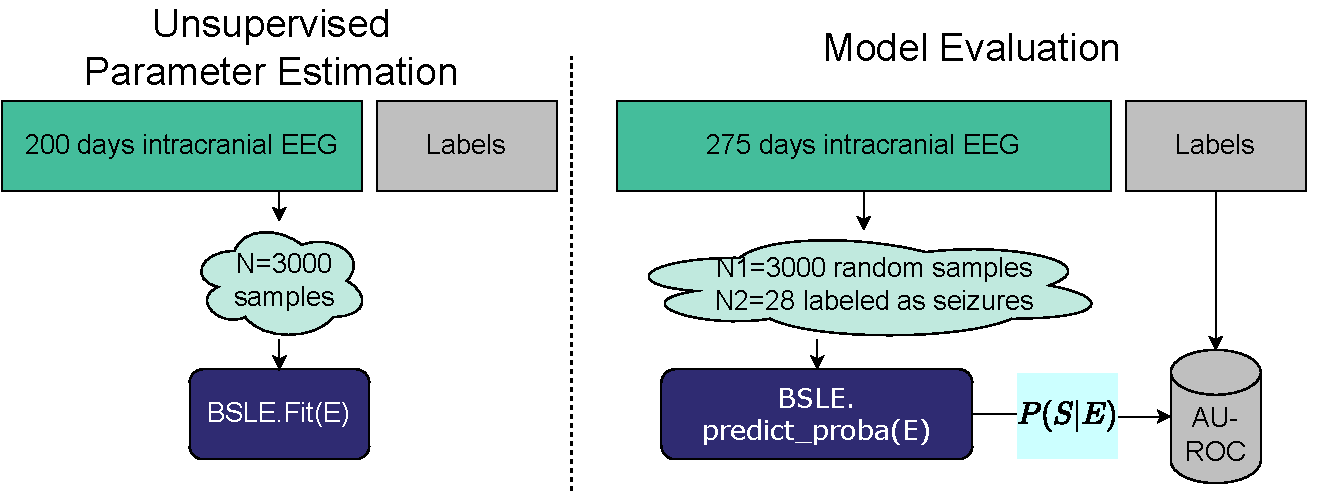
\includegraphics[width=\textwidth]{figs/unsupervised_study_scope.pdf}
    \label{fig:my_label}
    \caption{Scope of study}
    \end{figure}
}

\only<2>{
    \begin{figure}
    \centering
    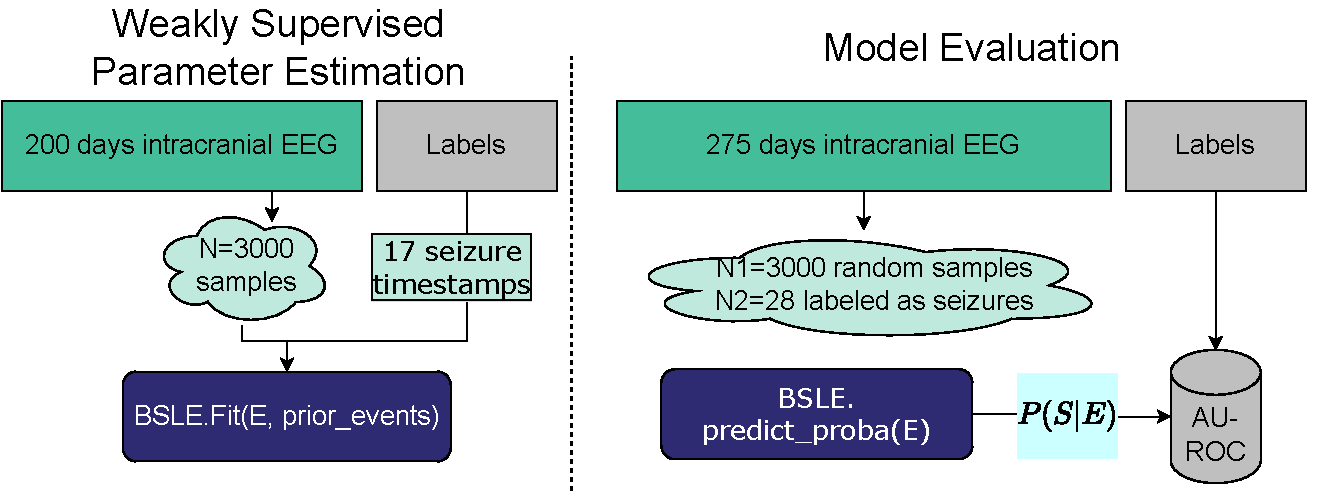
\includegraphics[width=\textwidth]{figs/weakly_supervised_study_scope.pdf}
    \label{fig:my_label}
    \caption{Scope of study}
    \end{figure}
}
    
\note[item]{We simulate a prospective study, which starts with an offline calibration phase, followed by an online validation phase.}
\note[item]{The separation of concerns ensures simulating a real-time setting, in which the 'offline' calibration phase is followed by an 'online' seizure detection mode.}
\note[item]{In the unsupervised study, we randomly sample 3000 segments of length 10 seconds each.}
\note[item]{We use these segments to estimate the parameters of the BSLE model.}
\note[item]{Next, we take all the seizures from the validation data, along with 3000 randomly sampled segments. We apply the BSLE estimation to each sample independently, to produce seizure probabilities.}
\note<2->[item]{In the weakly supervised version, we allow the option of appending a list of time stamps during which a past seizure occurred. These can be gained from clinical labels as well as self-reported seizure records.}
\note<2>[item]{In this case, a cyclical 24-hour prior function is provided based on domain knowledge.}

\end{frame}

%%%%%%%%%%%%%%%%%%% Pipeline %%%%%%%%%%%%%%%
\begin{frame}{Methods}
    \begin{figure}
        \centering
        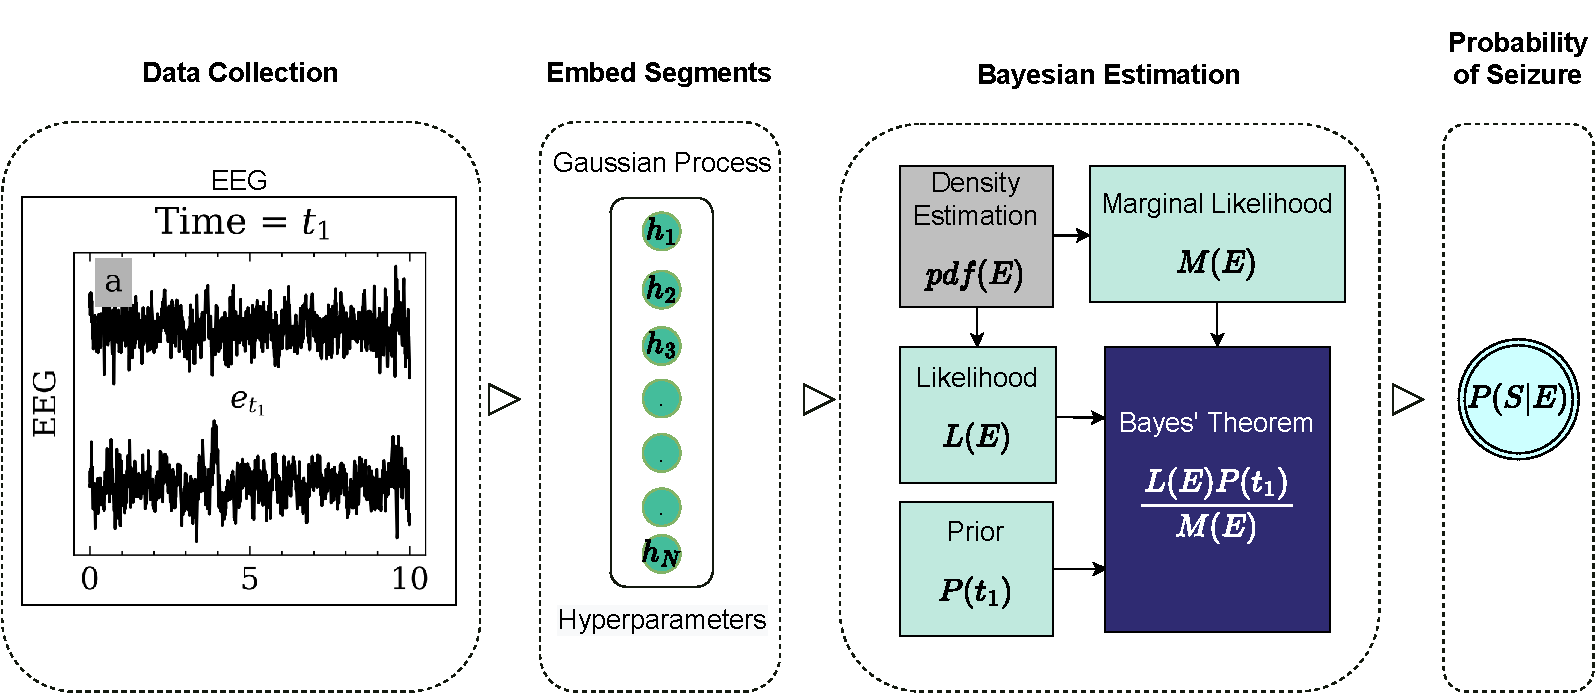
\includegraphics[width=\textwidth]{figs/pipeline.pdf}
        \caption{Bayesian Seizure Likelihood Estimation (BSLE) pipeline}
        \label{fig:my_label}
    \end{figure}

        \note[item]{Our method composes two stages: First, the EEG distribution is modeled and is used to assign novel sequences higher seizure likelihoods. Then, a priori knowledge based on the time covariate is added for supervised improvements.
        \item Weakly Supervised Bayesian Estimation of Seizure Likelihood}
\end{frame}


%%%%%%%%%%%%%%%%%%% Embeddings %%%%%%%%%%%%%%%
\subsection{Embedding EEG}

\begin{frame}{Embedding EEG Segments, by}

\begin{columns}[T] % T specifies that the columns should be top-aligned
    
    \begin{column}{0.618\textwidth} % specifies the width of the left column

    \begin{block}{Maximizing the likelihood of:}
        % Maximize the likelihood of:
        $$e(t_1) \sim \mathcal{GP}(m(t), k(t, t'))$$
        % where (reminder):
        $$m(t) := \mathbb{E}[e(t)]$$
        $$k(t, t') := \mathbb{E}[(e(t) - m(t))(e(t') - m(t'))]$$
    \end{block}
    
    \end{column}
    
    \begin{column}{0.382\textwidth} % specifies the width of the right column
    \vspace{-\baselineskip}
    \begin{figure}
        \centering
        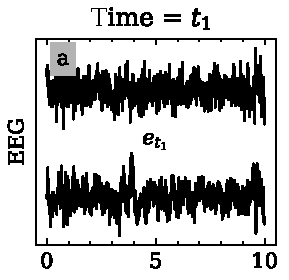
\includegraphics[width=\textwidth]{figs/eeg_sample.pdf}
        \label{fig:my_label}
    \end{figure}
    
    \end{column}
\end{columns}
    \vspace{-\baselineskip}
    \begin{block}{subject to:}
        \begin{itemize}
            \item $e(t_1)$ is a given z-scored EEG segment.
            \item $m \equiv 0$.
            \item $k \equiv K_{Matern}(\frac{3}{2})$.
        \end{itemize}
    \end{block}

\note[item]{A Gaussian process defines a distribution over functions of a continuous space, in our case over time from 0 to 10 seconds.}
\note[item]{A GP can be fully specified by a mean function and a covariance kernel.}
\note[item]{The first step of our process is to embed the high dimensional time series into a low dimensional representation.}
\note[item]{The embeddings are learned via gradient descent on a variational lower bound. Maximizing this ensures that the Gaussian Process parameters learned are those that maximize the log-likelihood of the observed data.}

\end{frame}

\begin{frame}{Learned embeddings}

    \begin{columns}
        \begin{column}{0.382 \textwidth}
            \begin{block}{$e_{t_1} \underset{ELBO}{\longmapsto} h_{t_1}$}
                Each sample ($d=800$) gets mapped to :

                \begin{itemize}
                    \item signal covar. $K_{data}$
                    \item task covar. $K_{tasks}$
                    \item obs. noise $\vec{\epsilon}$
                \end{itemize}
                parameters ($d=8$) \\ which maximize:
                $$p(f(e_{t_1}) \mid h_{t_1})$$
            \end{block}
        \end{column}
        \begin{column}{0.618 \textwidth}
                    
            \begin{figure}
                \centering
                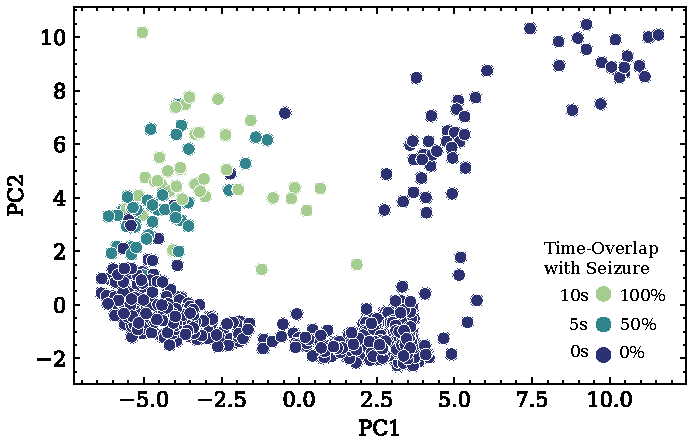
\includegraphics[width=\textwidth]{figs/embeddings_double.pdf}
                \caption{EEG embeddings}
                \label{fig:my_label}
            \end{figure}
        \end{column}
    \note[item]{Each point represents a 10-second EEG segment fit with a Gaussian process.}
    \note[item]{The parameters of the Gaussian Process consist of three types: data covariance kernel, task covariance kernel, and observational noise parameters.}
    \note[item]{The full kernel will be something like $K_{data} \otimes (covar\_factor * covar\_factor^{T} + diag(softplus(raw\_var))$, to which $softplus(raw\_noise)$ is added as a diagonal component. In some sense, the raw\_var parameter captures the task dependent noise. The likelihood noise is indeed somewhat redundant, but is important because it distinguishes between observations $e_t$ and the latent function f.}
        
    \end{columns}

\end{frame}


%%%%%%%%%%%%%%% Estimating Seizure LIkelihood %%%%%%%%%%%
\subsection{Estimating Seizure Posterior Probability}

\begin{frame}{Estimating densities $pdf_E(h)$}
\begin{columns}[t]
    \begin{column}{0.382\textwidth}
       
    \begin{figure}
            \centering
            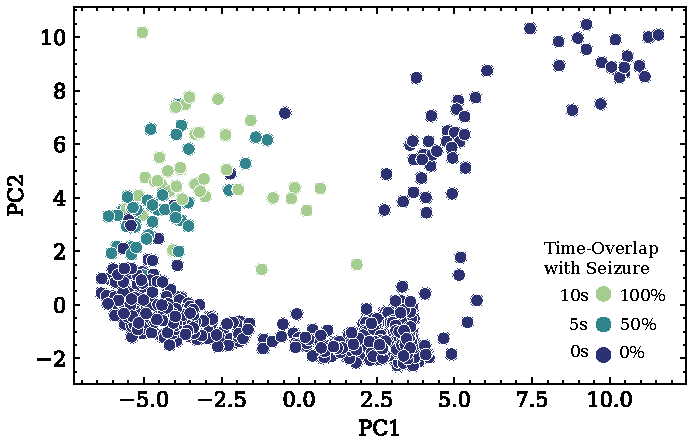
\includegraphics[width=\textwidth]{figs/embeddings_double.pdf}
            \caption{Eight-dimensional embeddings preserve class separability.}
            \label{fig:my_label}
        \end{figure}        
    \end{column}
    \begin{column}{0.618\textwidth}

    \begin{figure}
            \centering
            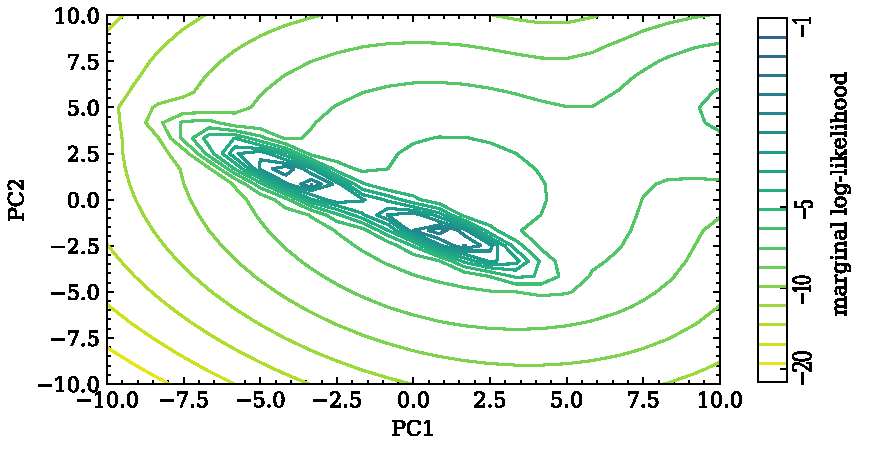
\includegraphics[width=\textwidth]{figs/de_pc1_pc2.pdf}
            \caption{Estimating $\hat{pdf_E}(h)$ with Gaussian mixture model}
            \label{fig:my_label}
        \end{figure}
        
        
    \end{column}
    \end{columns}

    \note[item]{So, now we have a set of 8-dimensional vectors, such that seizures are distinguishable from non-seizures.}
    \note[item]{The next step is to es}
    \note[item]{GMM with 4 components was fit to a 5 dimensional }
    
\end{frame}


\begin{frame}{Highest density regions}

    \begin{columns}[T] % T specifies that the columns should be top-aligned
    
    \begin{column}{0.382\textwidth} % specifies the width of the left column
    
        \begin{figure}
        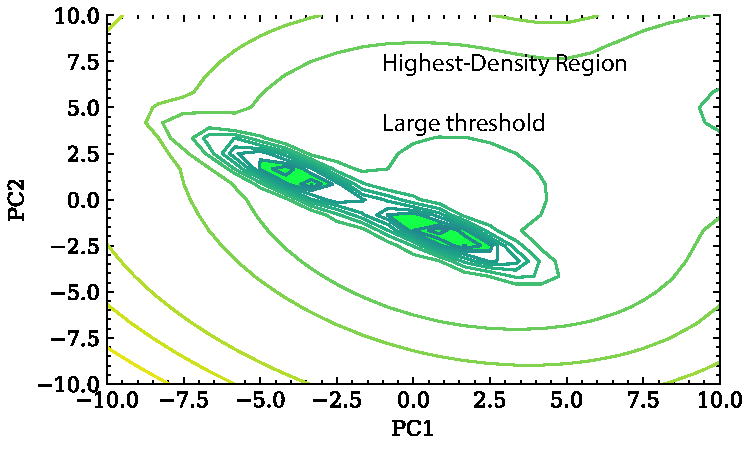
\includegraphics[width=\textwidth]{figs/de_pc1_pc2_likelihood_hdr_large_threshold.pdf}
    \end{figure}
    \end{column}
    
    \begin{column}{0.618\textwidth} % specifies the width of the right column
    \onslide<1->{
        \begin{figure}
            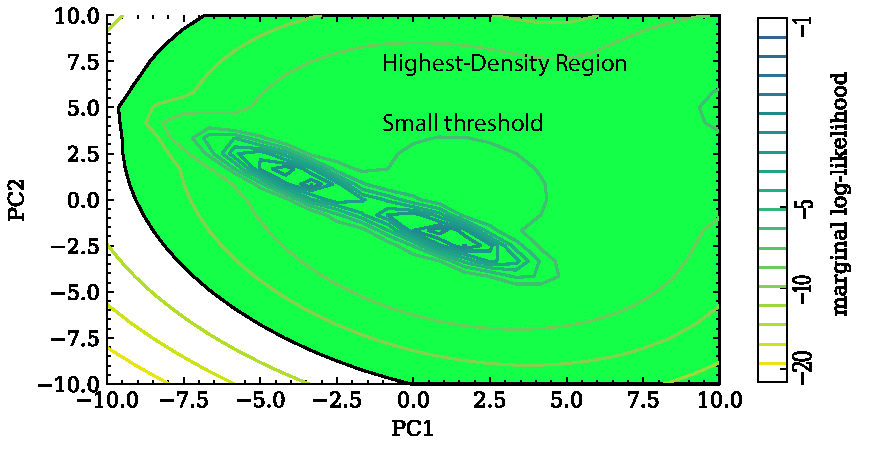
\includegraphics[width=\textwidth]{figs/de_pc1_pc2_likelihood_hdr_small_threshold.pdf}
        \end{figure}
    }
    \end{column}
    
    \end{columns}
    \begin{definition}[$\alpha$- Highest density region]
        \begin{equation*}
            R(f_\alpha) = \{ x : f(x) \geq f_\alpha \},
        \end{equation*}
        $f_\alpha$ is the largest constant such that $\prob(X \in R(f_\alpha)) \geq 1-\alpha$
    \end{definition}

    \note[item]{Highest density regions are regions in a space, such that a specific proportion of the mass lies within the region.}
    \note[item]{For example on the left, when we choose a low $\alpha$, a low threshold for the highest density region, we get two small peaks which account for about 10 percent of the total mass.}
    \note[item]{On the example on the right, we choose a high $\alpha$, so we get a large region which accounts for about 90 percent of the mass.}
    \note[item]{Now, this threshold $\alpha$ is a hyperparameter of the model. But let's assume it's fixed for the next slide, at a relatively low threshold, between 5 and 10 percent.}
\end{frame}

\begin{frame}{Likelihood function}
    \begin{figure}
        \centering
        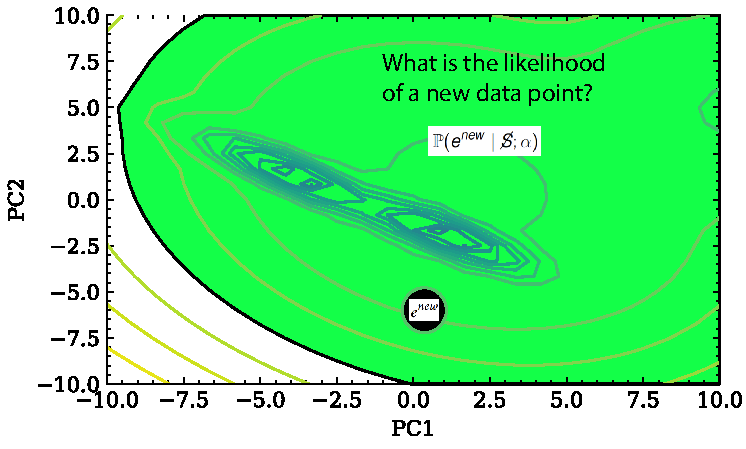
\includegraphics[width=0.9\textwidth]{figs/de_pc1_pc2_likelihood_likelihood_small_threshold_intro.pdf}
        % \caption{Caption}
        \label{fig:my_label}
    \end{figure}
    \note[item]{The green is the 0.05 highest density region.}
\end{frame}

\begin{frame}{Likelihood function}


    \begin{columns}[T] % T specifies that the columns should be top-aligned
    
    \begin{column}{0.5\textwidth} % specifies the width of the left column
    
        \begin{figure}
        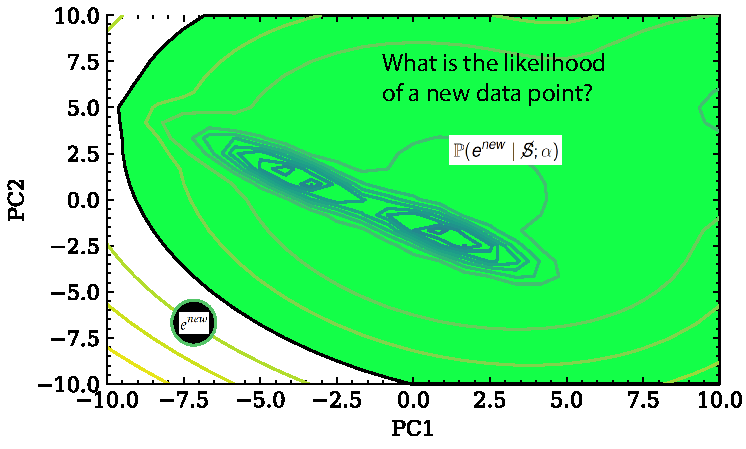
\includegraphics[width=\textwidth]{figs/de_pc1_pc2_likelihood_likelihood_small_threshold_answer_outside.pdf}
    \end{figure}

    \end{column}
    \begin{column}{0.5\textwidth} % specifies the width of the right column
        \begin{figure}
            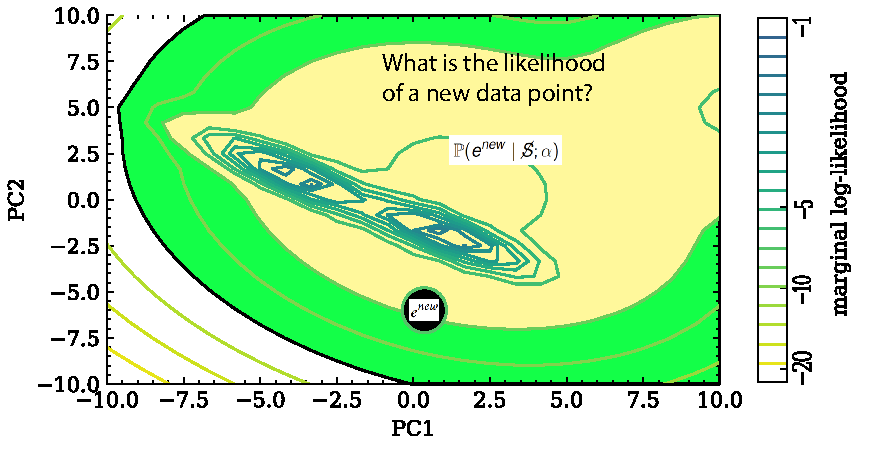
\includegraphics[width=\textwidth]{figs/de_pc1_pc2_likelihood_likelihood_small_threshold_answer_inside.pdf}
        \end{figure}
    \end{column}

    \end{columns}

    \begin{definition}[BSLE likelihood]
        \begin{equation*}
        \label{eq:c3bsle:likelihood}
        L_{\cancel{S}}(e^{new)} = 
        \prob(e^{new} \mid \cancel{S} ; \alpha) = \begin{cases}0 &\text{if $e^{new} \notin HDR_\alpha$} \\
        \mathcal{Z}(e^{new}) &\text{if $e^{new} \in HDR_\alpha$}
        
        \end{cases}
        \end{equation*}
    \end{definition}
    
\end{frame}

\begin{frame}{Marginal Likelihood}

    \begin{columns}[T] % T specifies that the columns should be top-aligned
    
    \begin{column}{0.55\textwidth} % specifies the width of the left column

    \begin{definition}[BSLE marginal likelihood]
    \begin{equation*}
    \label{eq:c3bsle:evidence}
    \prob(E) = \prob(\{pdf(e) \leq pdf(E)\})
    \end{equation*}
    \end{definition}
    
    \begin{block}{Geometric meaning}
        The probability of observing a sample $e^{new}$, is equal to the purple region divided by the entire region. 
    \end{block}
    
    \end{column}
    
    \begin{column}{0.45\textwidth} % specifies the width of the right column
    \begin{figure}
        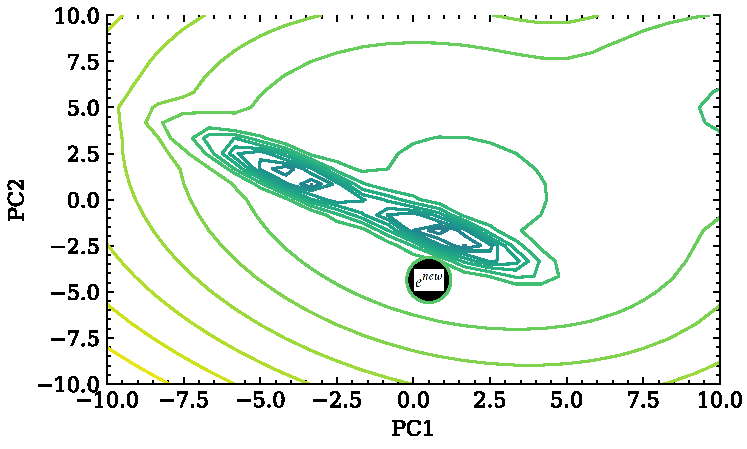
\includegraphics[width=\textwidth]{figs/de_pc1_pc2_likelihood_e_new.pdf}
    \end{figure}

        \begin{figure}
            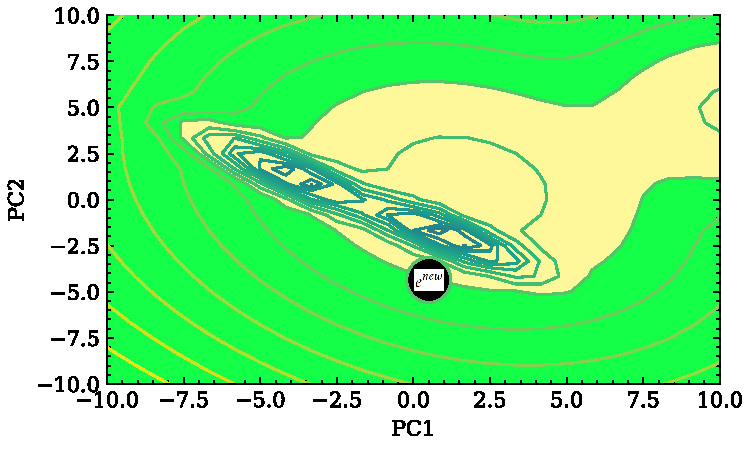
\includegraphics[width=\textwidth]{figs/de_pc1_pc2_likelihood_e_new_boundary.pdf}
        \end{figure}
    
    \end{column}
    
    \end{columns}
    \note[item]{The essence of the novelty score $\mathcal{Z}(e^{new})$ is that it maps data samples to the interval $[0,1]$, such that more anomalous samples (i.e. samples from less dense regions) are given larger values.}
    \note[item]{We adopt quantiles as a way of measuring risk.}
    \note[item]{For a fixed constant $0<p<1$, the $p$-quantile of a continuous random variable is a constant $\zeta$ such that $p$ of the distribution's mass lies below $\zeta$.}
    \note[item]{For example, the median is the 0.5-quantile.}
    \note[item]{The method used here is called Quantile estimation with Monte Carlo Sampling.}
\end{frame}


\subsubsection{Bayesian Estimation}
\begin{frame}{Estimate seizure likelihood with Bayes' theorem}
    
    \begin{alertblock}{Goal}
        $$\mathbb{P}(S_t \mid E_t) = \frac{\mathbb{P}(E_t \mid S) \mathbb{P}(S_t)}{\mathbb{P}(E_t)} = \frac{L(E_t)P(t)}{M(E_t)}$$
    \end{alertblock}

    \pause
    \begin{block}{Equivalent goal}
        \vspace{-\baselineskip}
        $$\mathbb{P}(S_t \mid E_t) = 1 - \mathbb{P}(\cancel{S_t} \mid E_t) = 1 - \frac{\mathbb{P}(E_t \mid \cancel{S}) \mathbb{P}(\cancel{S}_t)}{\mathbb{P}(E_t)} = 1 - \frac{L_{\cancel{S}}(E_t)P_{\cancel{S}}(t)}{M(E_t)}$$
    \end{block}

    \pause
    \begin{block}{Method overview}
        \begin{enumerate}[<+->]
            \item $M(E_t)$ is the likelihood of observing $E_t$ in general.
            \item $L_{\cancel{S}}(E_t)$ is the likelihood of observing $E_t$ provided $\cancel{S}$.
            \item $P_{\cancel{S}}(t)$ is chosen to model the temporal seizure patterns.
        \end{enumerate}
    \end{block}

    \note[item]{$L(E_t)$ and $M(E_t)$ are computed with Monte Carlo Quantile Estimation. The likelihood is the quantile of the sample, trimmed at the HDR_\alpha boundary.}
    \note[item]{$P(t)$ is a prior function which relies only on the time covariate.}
    \note[item]{! Write Equivalent goal on board}
\end{frame}



\begin{frame}<1-3>{Priors}
    \begin{columns}
    \begin{column}{0.55\textwidth}
        \onslide<1->{
        \begin{block}{Uniform prior}
            $$\prob(S_t) = \lambda_0 \cdot T$$
        \end{block}
        }
        \onslide<2->{
        \begin{block}{Circadian prior}
            \begin{align*}
            f(x | \mu, \kappa ; \omega) = \frac{\exp (\kappa \cos (\omega (x - \mu)))}{2 \pi I_0(\kappa)}
            \label{eq:2background:vm_density}
            \end{align*}
        
            \begin{equation*}
            \prob(S_t) = \frac{1}{K}\sum_{i=0}^{23} f(t \mid i, k) 
            \end{equation*}

        \end{block}
        }
    \end{column}

    \begin{column}{0.45\textwidth}
        \onslide<2-3>
        \begin{block}{Circadian prior}
        \begin{figure}
            \begin{overprint}
            \onslide<2>
            \centering
            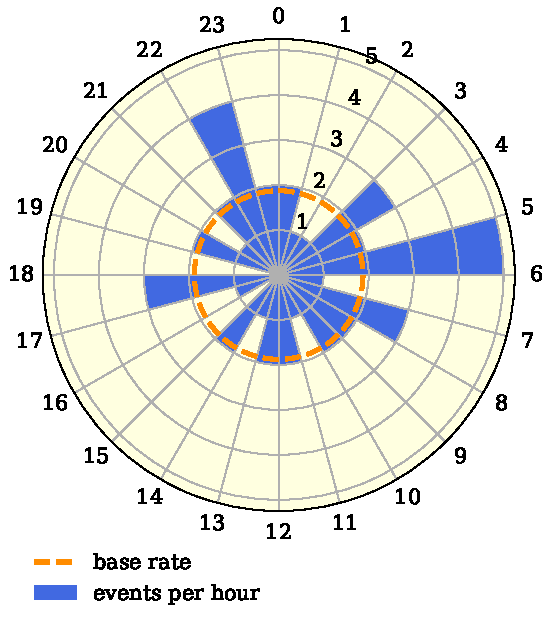
\includegraphics[width=\textwidth]{figs/polar_hist.pdf}
            \onslide<3>\centering
            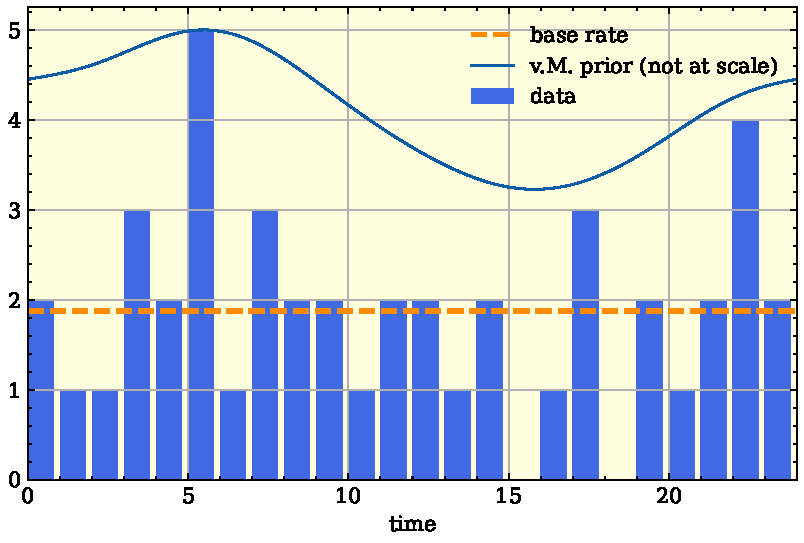
\includegraphics[width=\textwidth]{figs/vm_prior.pdf}
            \end{overprint}
        \end{figure}
        \end{block}
        
    \end{column}
    
    \end{columns}
    % \begin{block}{}
    %     Uniform prior on left. Circadian prior on right.       
    % \end{block}
    \note<1->[item]{The uniform prior is the simplest. It means I give equal weight to each time point. My knowledge does not increase or degrade at any point.}
    \note<2->[item]{Another option is to look at seizure cycles, which has been explored more in recent years.}
    \note<2->[item]{Following other works, we set the prior to be cyclical with the von Mises distribution. Where $K$ is a normalizing constant evaluated numerically (\texttt{np.trapz}).}
    \note<2->[item]{
        In this work, we set $\omega \gets \frac{2\pi}{24}$ to scale the period to 24-hours, and drop it from the notation for brevity in the following text.
        }
\end{frame}


\section{Empirical Results}
\begin{frame}<1,2,3>{Evaluating BSLE on validation data}
    \only<1> {
    \begin{figure}
        \centering
        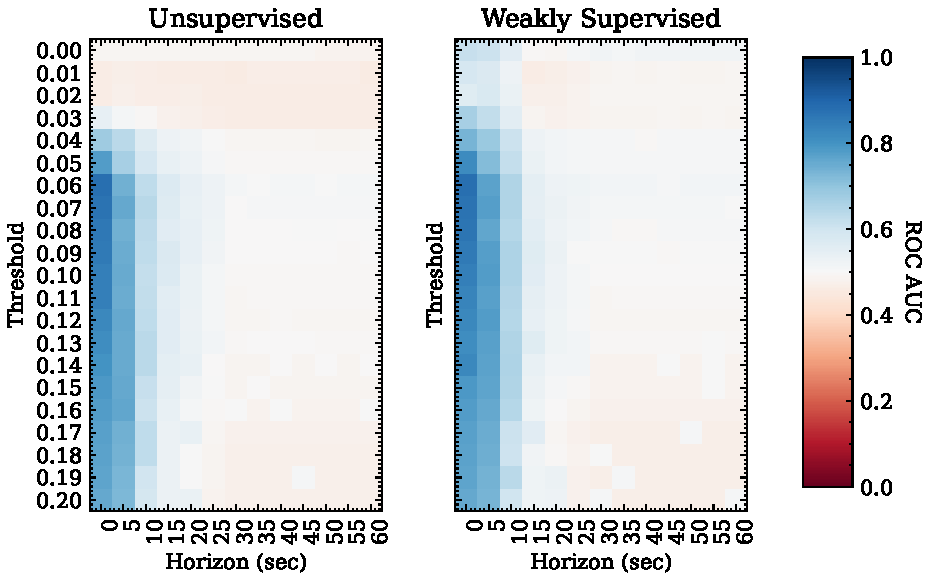
\includegraphics[width=0.95\textwidth]{figs/auc_roc_scores_for_thresholds_and_horizons_sec.pdf}
        % \caption{ROC-AUC on 3028 validation samples as a function of $\alpha$ and $\tau$}
        \label{fig:my_label}
    \end{figure}
    }
    \only<2> {
    \begin{figure}
        \centering
        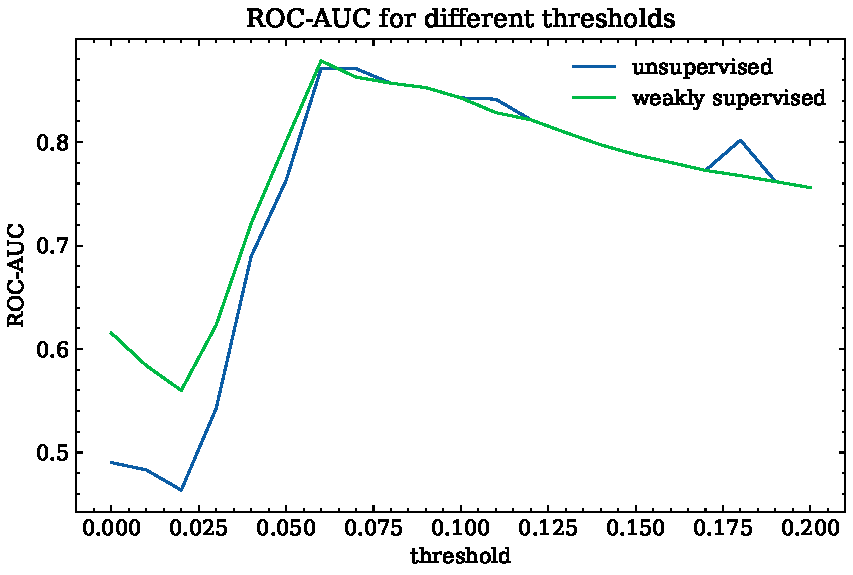
\includegraphics[width=0.95\textwidth]{figs/roc_auc_score_for_thresholds.pdf}
        % \caption{ROC-AUC on 3028 validation samples as a function of $\alpha$ and $\tau$}
        \label{fig:my_label}
    \end{figure}
    }
    \only<3> {
    \begin{columns}

    \begin{column}{0.5\textwidth}
    \begin{figure}
    \begin{subfigure}{\linewidth}
    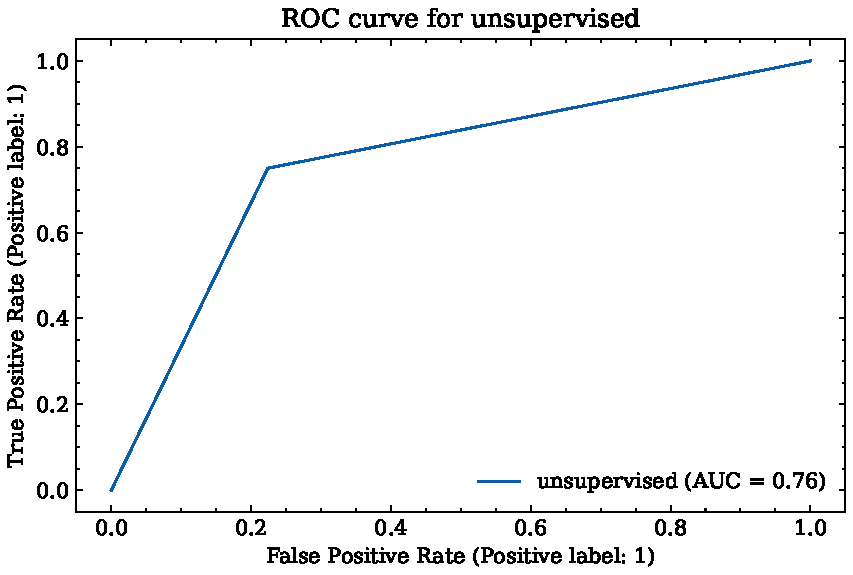
\includegraphics[width=\linewidth]{figs/roc_auc_unsupervised.pdf}
    % \caption{Figure 1}
    \end{subfigure}
    \end{figure}
    \end{column}

    \begin{column}{0.5\textwidth}
    \begin{figure}
    \begin{subfigure}{\linewidth}
    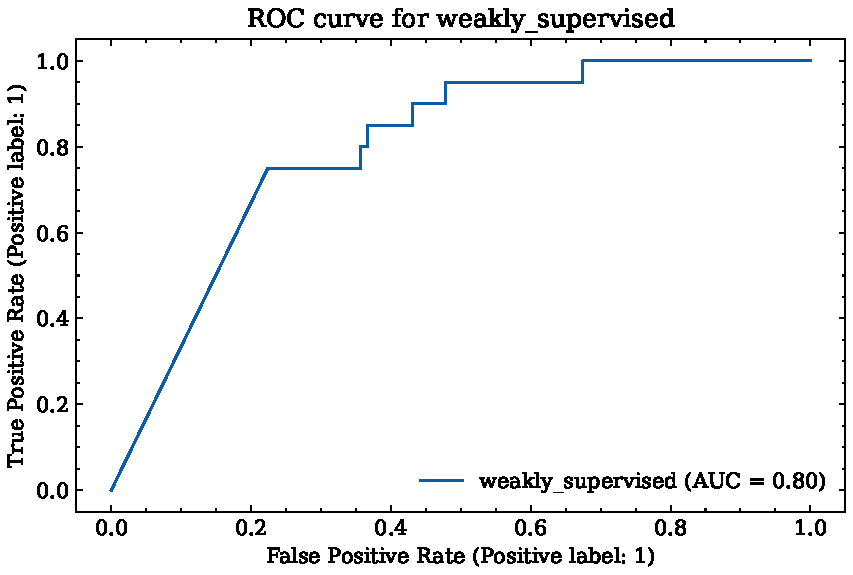
\includegraphics[width=\linewidth]{figs/roc_auc_weakly_supervised.pdf}
    % \caption{Figure 2}
    \end{subfigure}
    \end{figure}
    \end{column}
    % \caption{ROC curves for $\alpha=0.5$ and $\tau=0$}
    \end{columns}
    }
    \note<1->[item]{AUC-ROC scores smoothly distributed in the hyper-parameter space of both the unsupervised and weakly-supervised models, showing a low risk of over-fitting}
    \note<1->[item]{The lower region of $\alpha$ is }
\end{frame}


\section{Conclusion}
\begin{frame}{Conclusion}

    \begin{block}{}
        We present BSLE - a Bayesian Seizure Likelihood Estimator.
    \end{block}
    \pause
    \begin{block}{}
        BSLE uses a novelty score to model the likelihood that a siezure is not occurring, and a temporal prior to induce bias based on labels, if available.
    \end{block}
    \pause
    \begin{block}{}
        BSLE can be used for unsupervised seizure alerts, and in addition learn from untaped seizures.
    \end{block}
    \pause
    \begin{block}{}
    More work is required to statistically validate findings. Further work could use BSLE as a pseudo-labeler module in self-supervised learning.
    \end{block}
	% \pause
	% \begin{block}{Main contributions}
	%      \begin{enumerate}
	%          \item we do not have to fix a total time
	%          \item likelihood maximization is equivalent to maximization of the expected future return
 % 	   \end{enumerate}
	% \end{block}
	% \pause
	% \begin{block}{}
	%      We can compute posteriors over actions, states, and the total time.
	% \end{block}
	% \pause
	% \begin{block}{}
	%      The full variety of existing inference techniques can be applied to solving MDPs.
	% \end{block}
	% \note[item]{The key step to our approach is to introduce a mixture of finite-time MDPs as a model that is equivalent to the original time-unbounded MPD but has two advantages: it allows us to formulate a likelihood proportional to the expected future return, and inference in the mixture model can efficiently be realized with a single synchronous forward-backward propagation without having to fix a finite total time in advance.}
\end{frame}

\begin{frame}<beamer>{End}
	\begin{center}
		{\Huge\calligra Thank You}
	\end{center}
\end{frame}

\begin{frame}
        \frametitle{References}
        % \nocite{*}
        % \printbibliography
        \bibliographystyle{abbrvnat}
        \bibliography{refs}
\end{frame}


\appendix

\begin{frame}{Apx. 1 - Gaussian processes}

    \begin{definition}[Gaussian process]
        $$f(t) \sim \mathcal{GP}(m(t), k(t, t')$$
        where
        $$m(t) = \mathbb{E}[f(t)]$$
        $$k(t, t') = \mathbb{E}[(f(t) - m(t))(f(t') - m(t'))]$$
    \end{definition}
    \pause
    \begin{definition}[Matérn class of covariance functions]
        $$k_{Matern}(t, t') := \frac{2^{1-\nu}}{\Gamma(\nu)}(\sqrt{2\nu}d)^\nu K_\nu (\sqrt{2\nu}d)$$
        where
        $$d = (t-t')^T \Phi^{-2} (t-t')$$
    \end{definition}

    \note[item]{A Gaussian process, defined by a mean function and covariance kernel function, with a Matérn kernel is a specific family of distribution over functions. Parameterized by <FILL IN>, the}
    
    \note[item]{$d$ is the distance between $t$ and $t'$ scaled by the \emph{lengthscale} parameter $\Phi$}
    \note[item]{$\nu$ is a smoothness parameter. In this work, it is taken to be $\frac{2}{3}$, which limits us to functions which are exactly once differentiable.}
    \note[item]{$K_\nu$ is a modified Bessel function. The modified Bessel function has the property of being rapidly decaying, which means that it falls off quickly as the distance between two points increases. }
    \note[item]{+++This property is important in the context of kernel-based machine learning algorithms because it allows the kernel function to effectively capture the local structure of the data, while ignoring irrelevant or noisy features that may be present in the data.}

\end{frame}


%%%%%%%%%%%%%%%%%%%%%%%%%%%

\begin{frame}<1-2>{Sample spaces}
\begin{columns}[t]
    \begin{column}{0.5\textwidth}
    \begin{block}{}
        \onslide<1->{
        Let:
        \begin{enumerate}
            \item {$e_t \sim E(t) \in \Omega_E = \mathbb{R}^{c \times N}$}
        \end{enumerate}
        a random EEG variable,
        }
        
        \bigskip
        \onslide<2->{
            and:
            \begin{enumerate}
                  \setcounter{enumi}{1}
                \item $s_t \sim S(t) \in \Omega_S = \{0, 1\}$
            \end{enumerate}
            a random Seizure variable.
        }
    \end{block}
    
    \end{column}
    \begin{column}{0.5\textwidth}

    \begin{figure}  
        \centering
        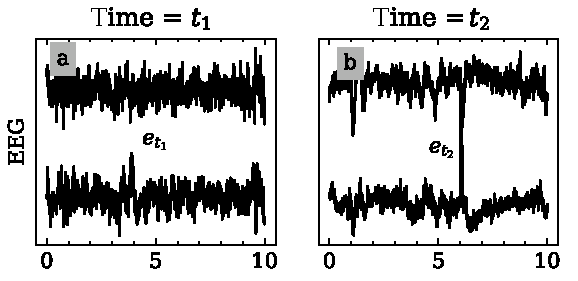
\includegraphics[width=\textwidth]{figs/sample_space_two_top_frames.pdf}
        \caption{Samples from $E(t_1)$ and $E(t_2)$.}
        \label{fig:my_label}

        \onslide<2->
        \centering
        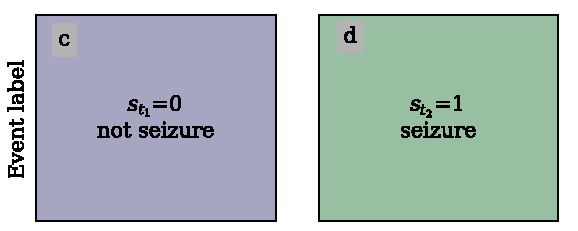
\includegraphics[width=\textwidth]{figs/sample_space_two_bottom_frames.pdf}
        \caption{Samples from $S(t_1)$ and $S(t_2)$}
        \label{fig:my_label}
    \end{figure}

        
    \end{column}
    \end{columns}

    \note<1->[item]{Defining a sample space and random variables.}


\end{frame}

\end{document}

% references
% https://www.cs.ubc.ca/~murphyk/Papers/dbnchapter.pdf